\section{わかるらんど}

わかるらんどはありとあらゆるフロー情報を非常に簡単に表示できるダッシュボードである。
わかるらんどの最大の特徴は、「スタンプ」によって人間の感情や現在の状況を極めて簡単に発信することができることである。
本章ではわかるらんどのユーザインタフェースと利用例について述べる。

\subsection{ユーザインタフェース}

図\ref{dashboard}図\ref{console}はわかるらんどのスクリーンショットである。
ユーザインタフェースは、ダッシュボード、投稿画面の2つからなる。
ダッシュボードと投稿画面はいずれも単一の画面で、上部のボタンで切り替えて利用する。
ダッシュボードには指定した情報を表示するウィジェット(図\ref{widget})を格子状に並べることができる。

ウィジェットには人間の感情や状態を表示するwakariウィジェットとセンサ情報などの数値を表示するdataウィジェットの2種類がある。
ウィジェットのバックグラウンドには人/物/現象の画像を表示し、その上に情報をオーバーレイで表示する。
情報はリアルタイムに更新が反映され、最新の情報のみを表示する。

投稿画面ではユーザとしてダッシュボードに投稿を行うことができる。
ユーザの投稿は「スタンプ」をクリックすることで行う。
スタンプは、
\begin{itemize}
\item 短いテキストをスタンプ化する
\item 画像のURL
\end{itemize}
の2つの方法で追加できる。
また、スタンプ投稿時にクリックの長さを変えることで、ダッシュボードにスタンプを表示する時間の変更が可能である。

\begin{figure}[h]
\centering
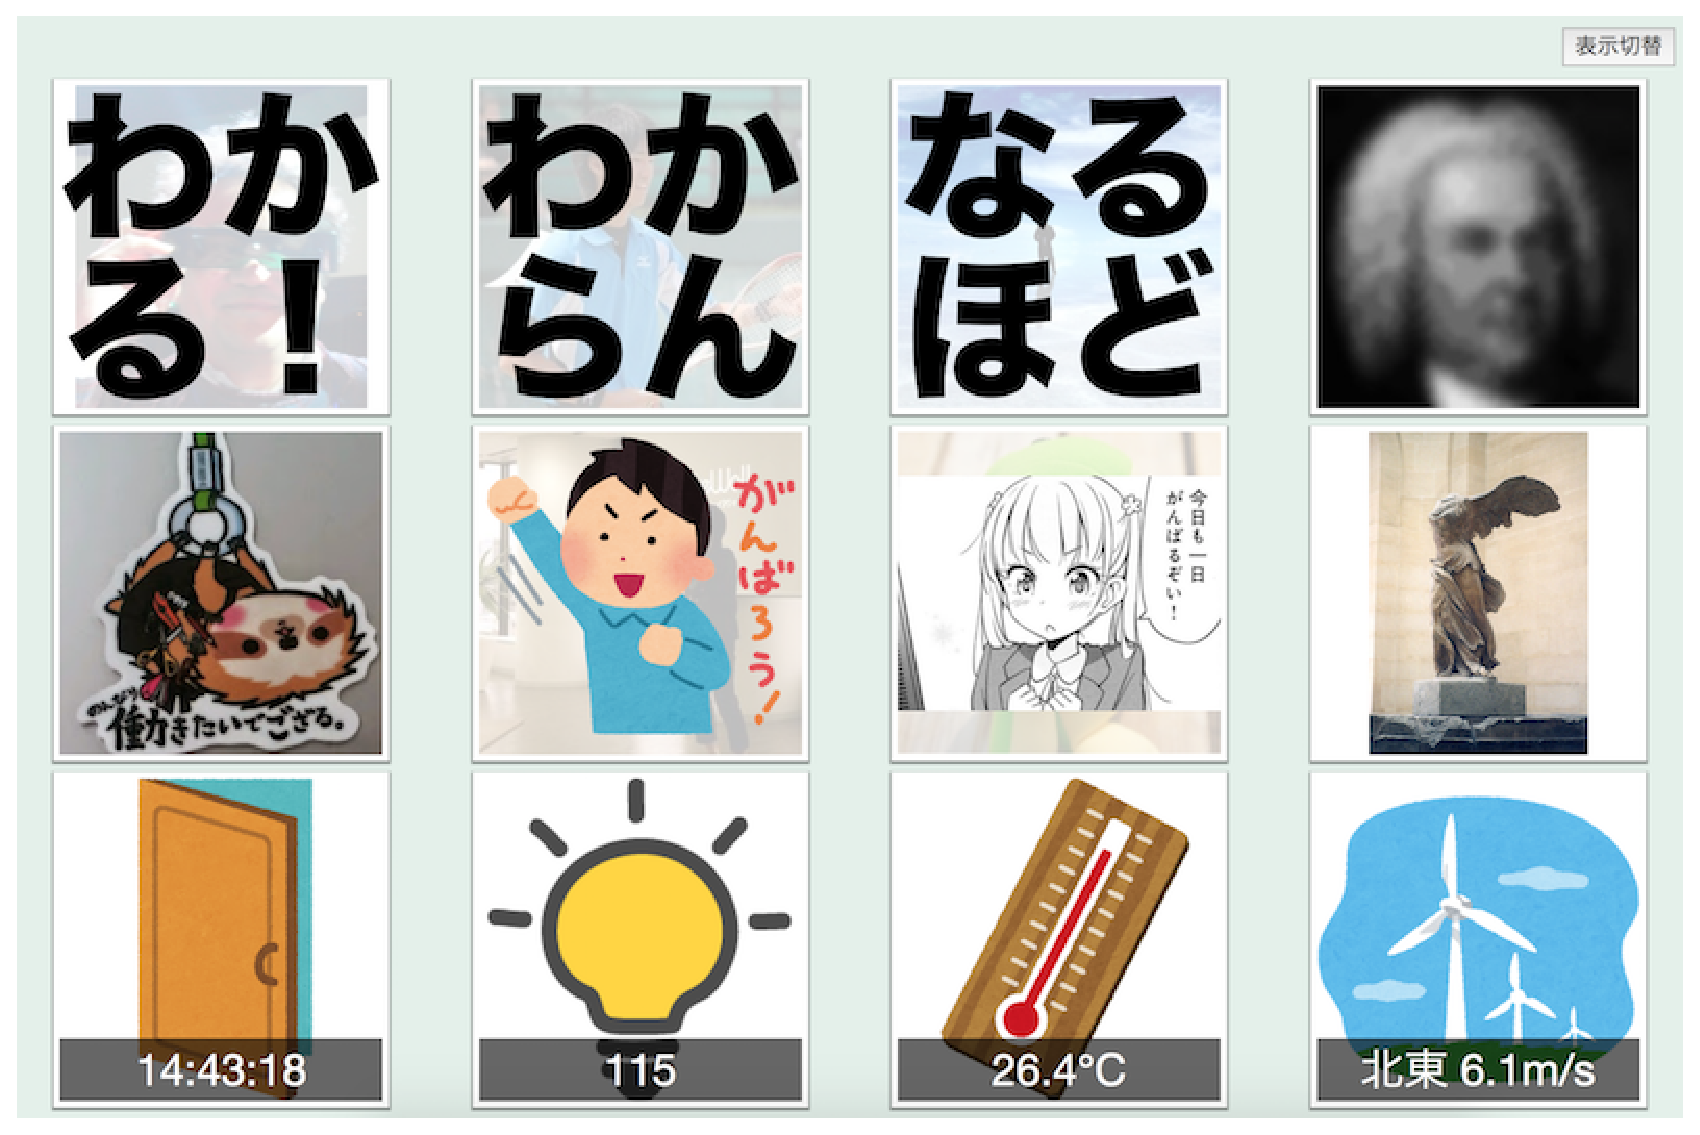
\includegraphics[width=7cm]{images/dashboard.eps}
\caption{わかるらんどのダッシュボード}
\label{dashboard}
\end{figure}

\begin{figure}[h]
\centering
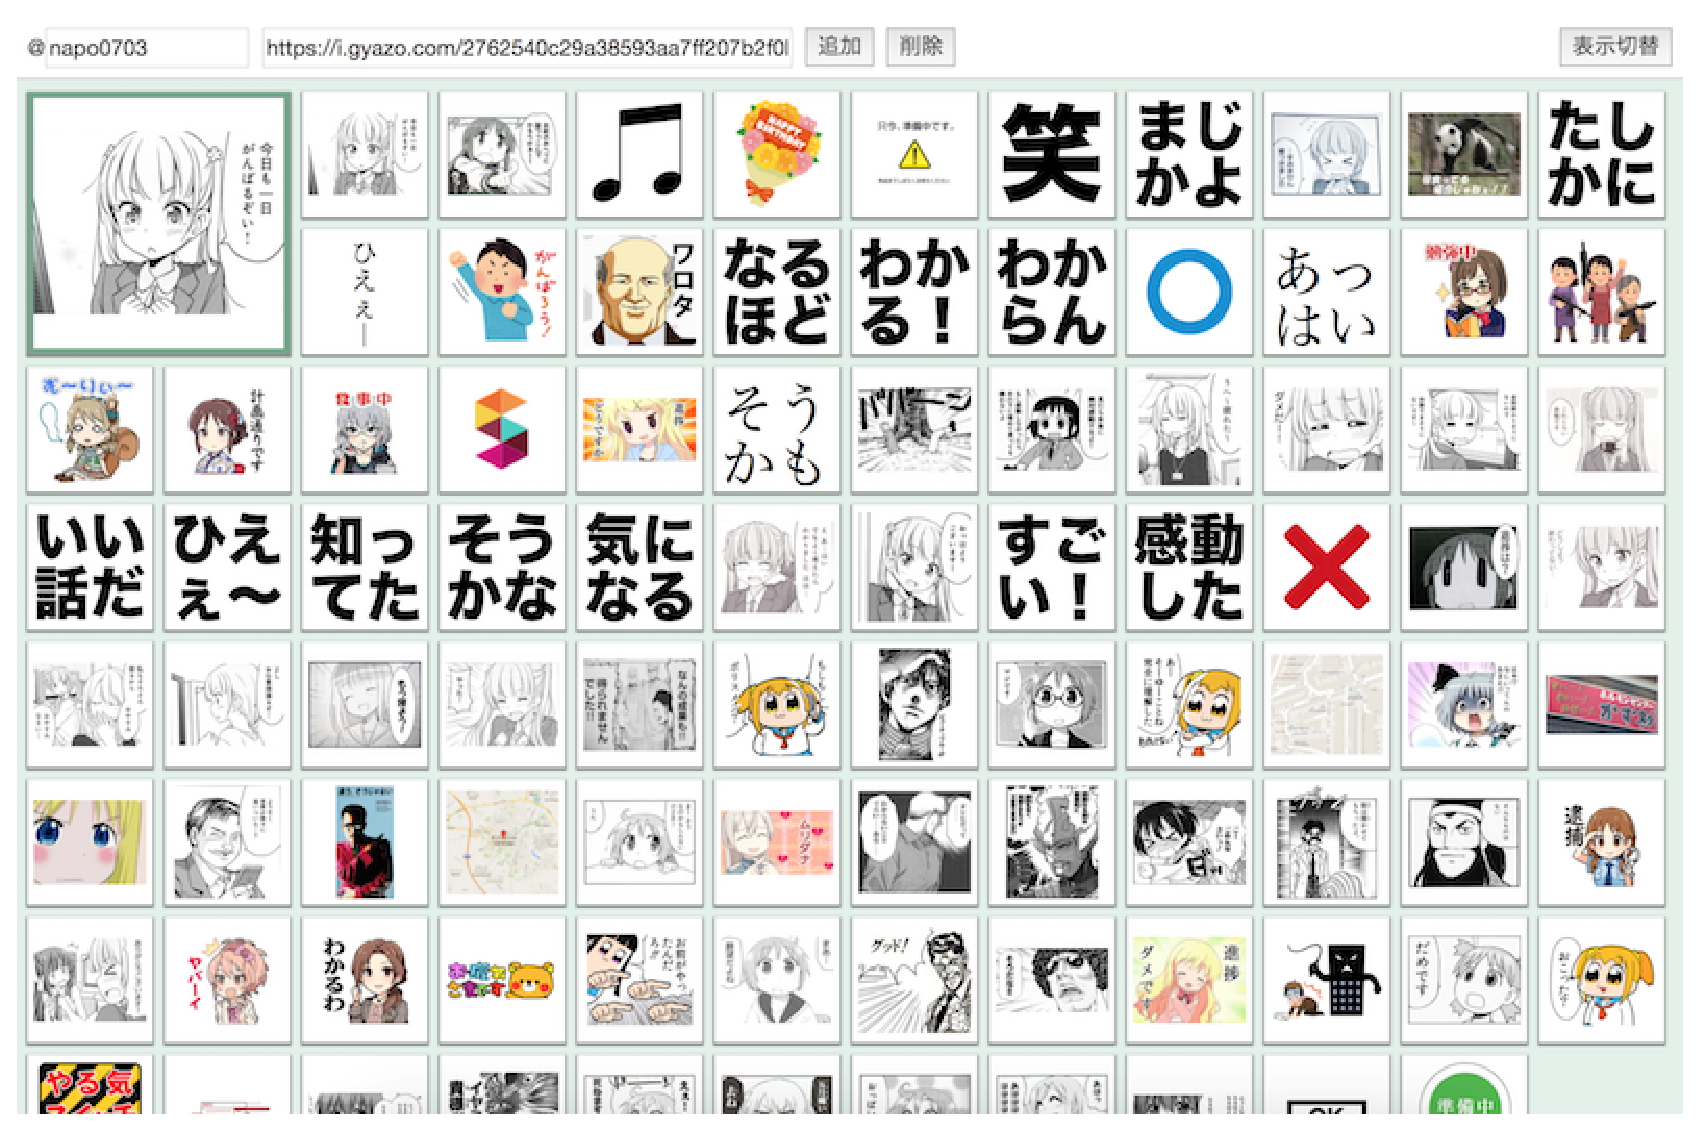
\includegraphics[width=7cm]{images/console.eps}
\caption{投稿画面}
\label{console}
\end{figure}

\begin{figure}[h]
\centering
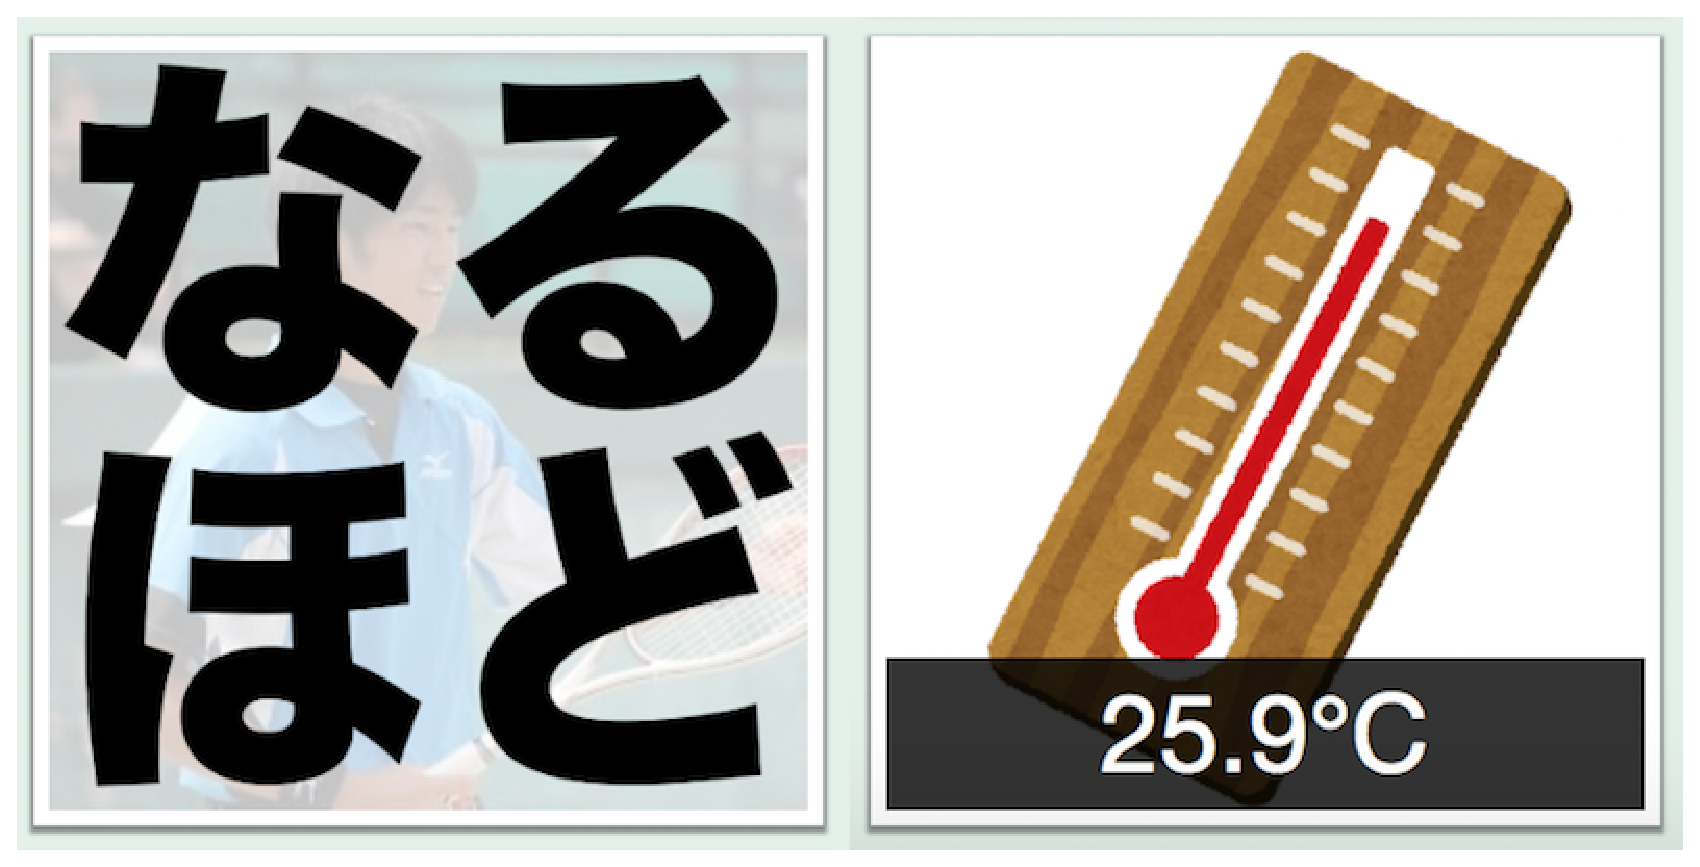
\includegraphics[width=7cm]{images/widget.eps}
\caption{wakariウィジェット(左)とdataウィジェット(右)}
\label{widget}
\end{figure}

\subsection{利用例}

\subsubsection{発表や講義での利用例}

図\ref{discussion}は講義や発表での利用例である。
これをサブスクリーンに表示することで、他の参加者の感情を把握したり登壇者が聴衆の反応を見ながら発表をすることができる。
また図\ref{vote}のようにアンケートを取ったり、図\ref{rescue}のように「寒い」「トイレに行きたい」など、
口頭では伝えにくい感情を周囲に伝えることもできる。

\begin{figure}[h]
\centering
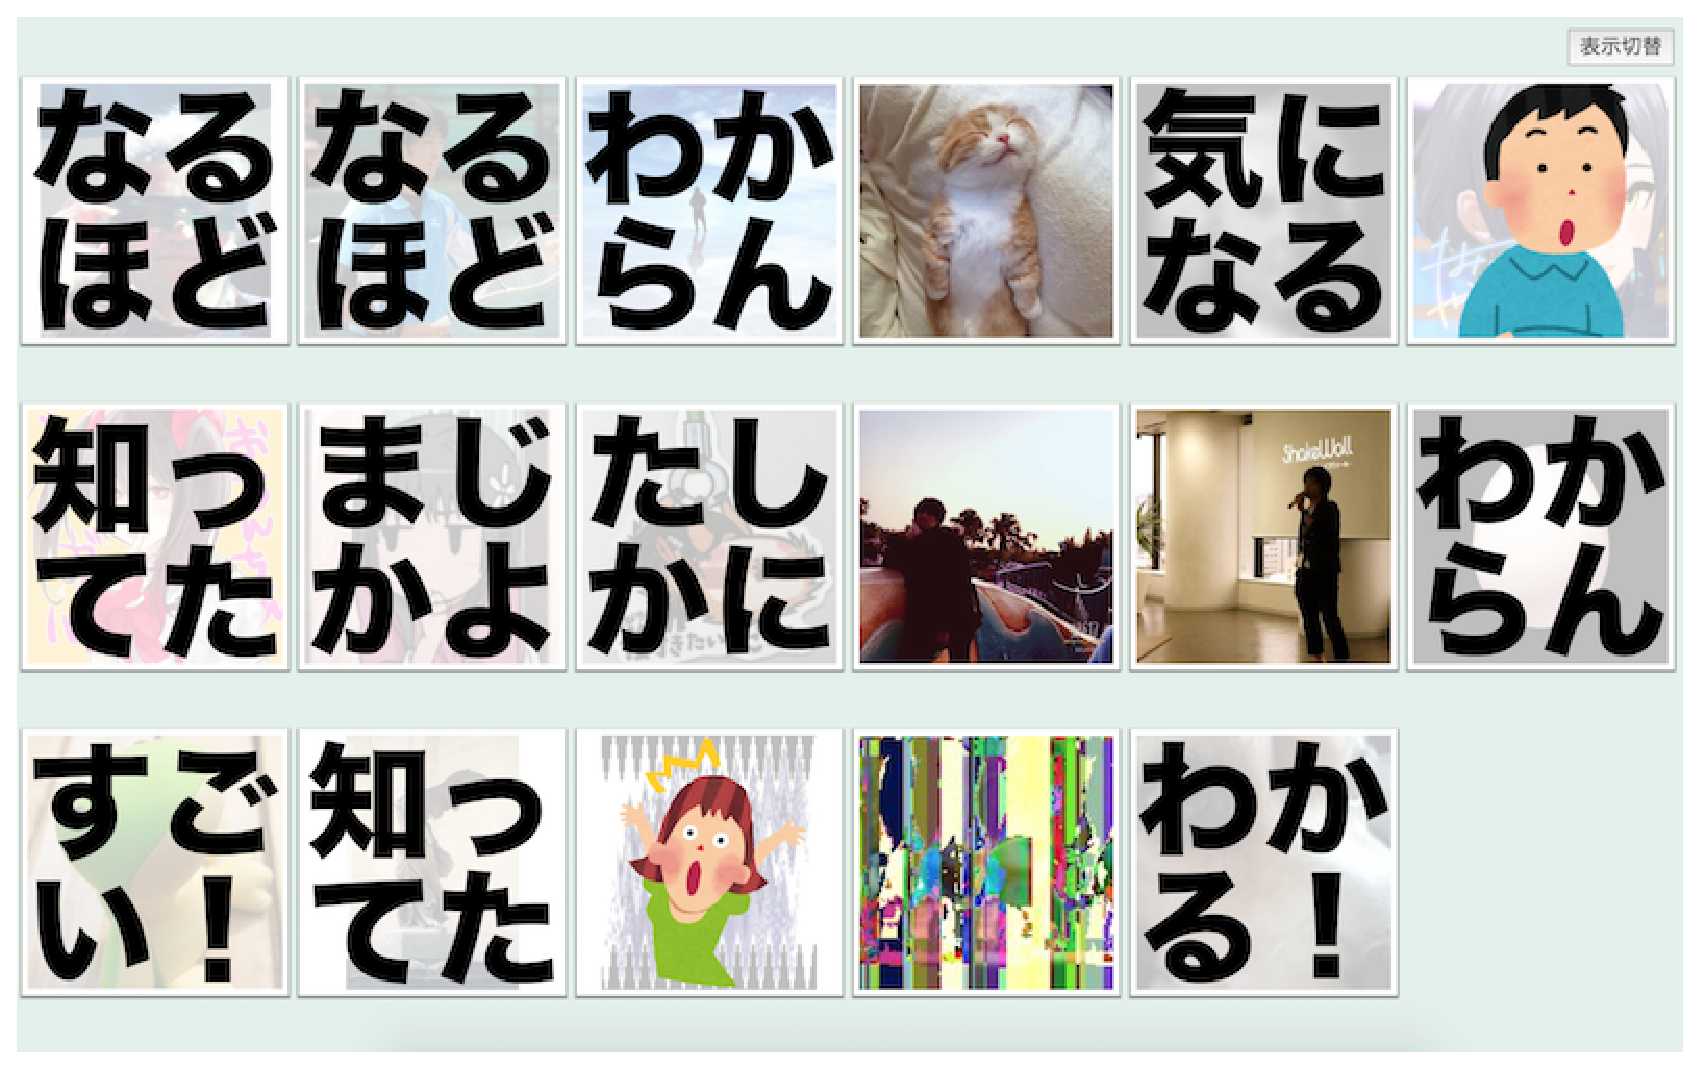
\includegraphics[width=7cm]{images/discussion.eps}
\caption{会議での利用}
\label{discussion}
\end{figure}

\begin{figure}[h]
\centering
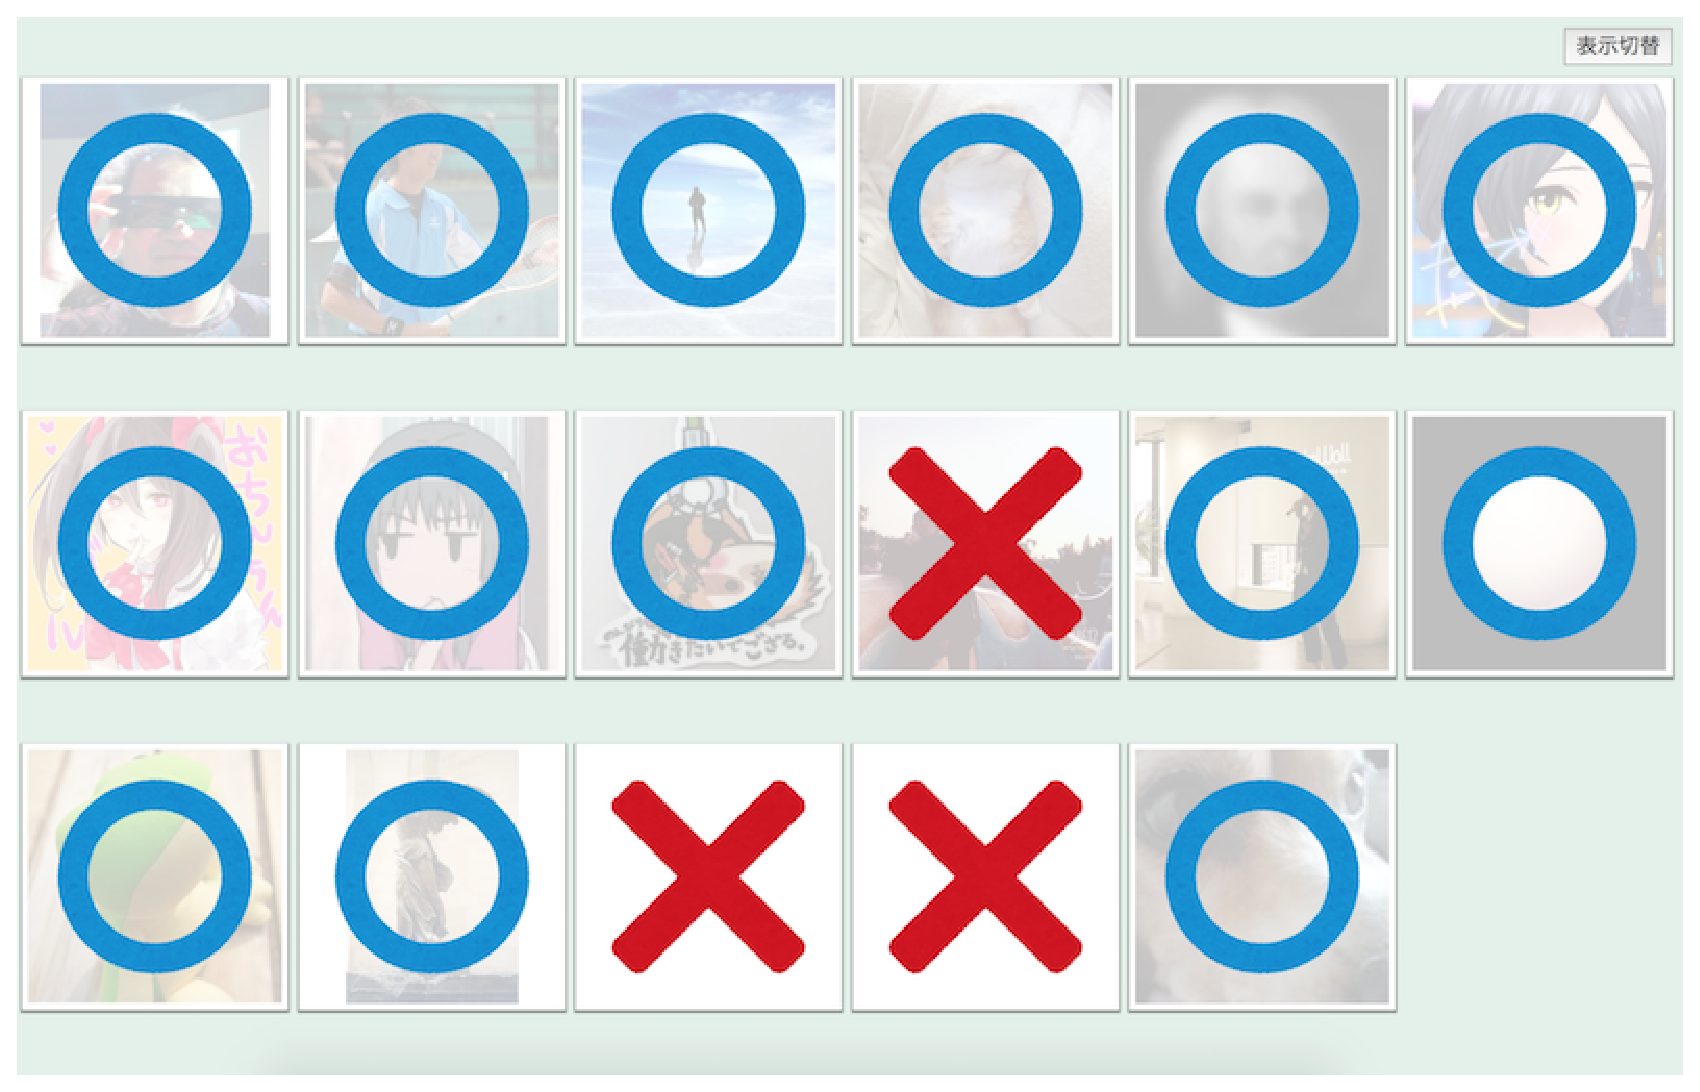
\includegraphics[width=7cm]{images/vote.eps}
\caption{アンケートとしての利用}
\label{vote}
\end{figure}

\begin{figure}[h]
\centering
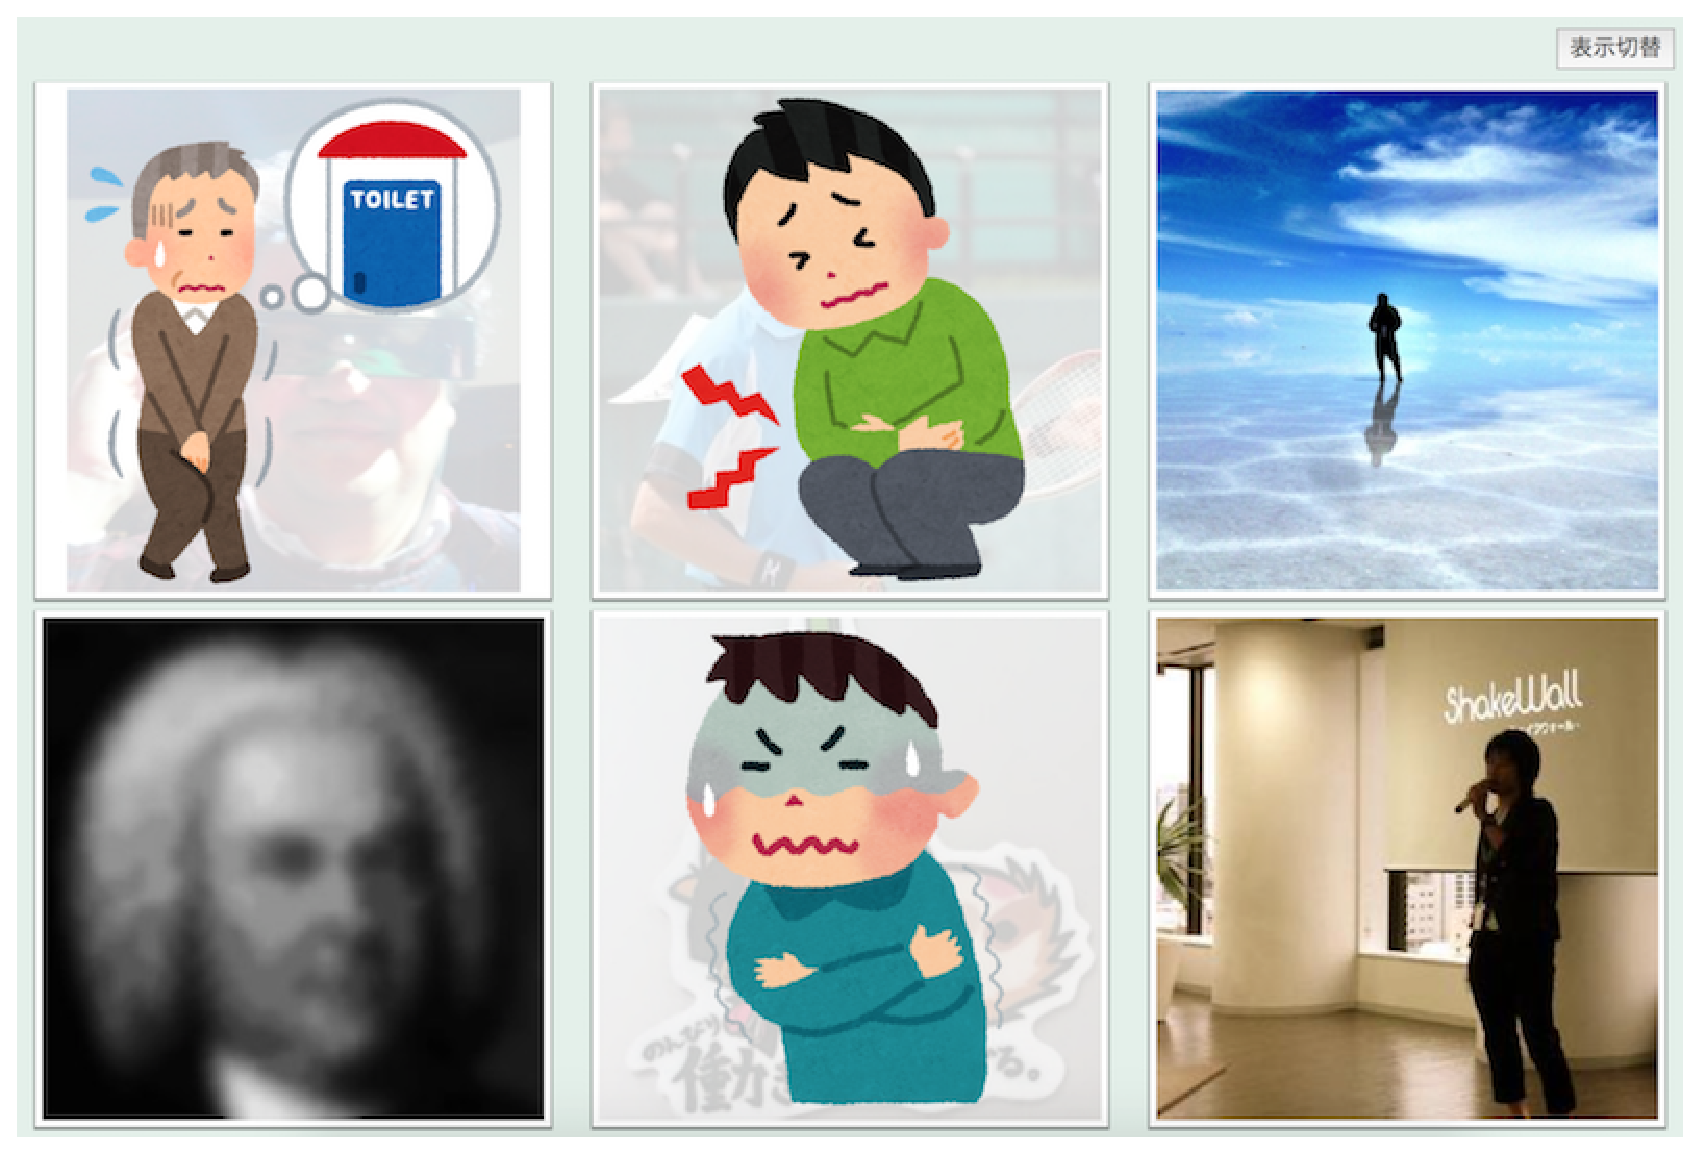
\includegraphics[width=7cm]{images/rescue.eps}
\caption{言い出しにくいことを伝える}
\label{rescue}
\end{figure}

\subsubsection{センサ情報等の表示}

図\ref{sensors}は、明るさ、ドアが最後に開いた時間、気温、風速、天気、メール未読件数、株価、電力使用量を表示した例である。
センサの値やインターネット上の情報、コンピュータの情報などをひと目で把握することができる。

\begin{figure}[h]
\centering
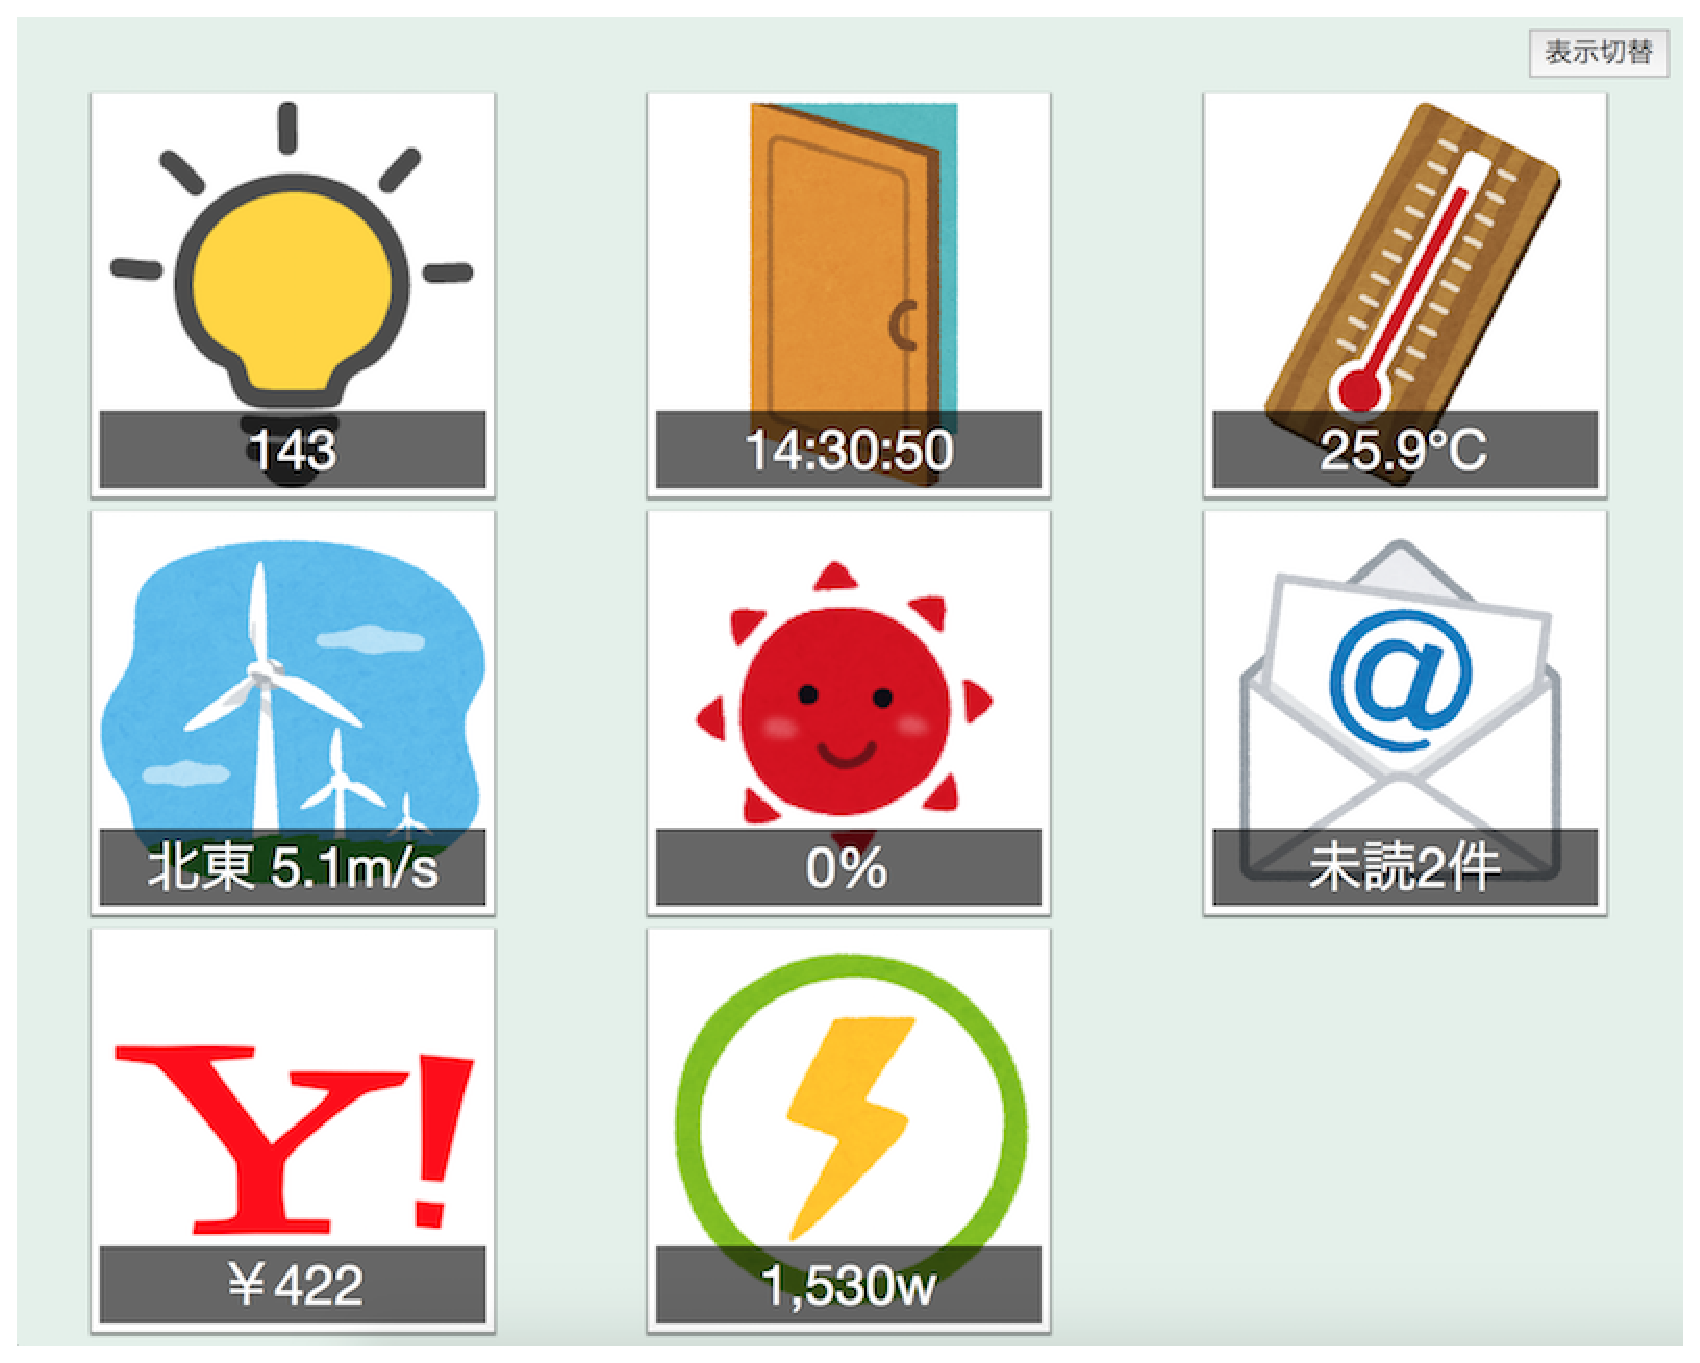
\includegraphics[width=7cm]{images/sensors.eps}
\caption{センサやWebの情報を表示}
\label{sensors}
\end{figure}

\subsubsection{家庭内サイネージ}

図\ref{home}は家庭での利用例である。
左上の夕食は家で食べるかという問いかけに対し、短いメッセージでを送ったり画像で返答することもできる。

また、ペットなど人間以外にセンサを取り付けて投稿させることも可能である。

\begin{figure}[h]
\centering
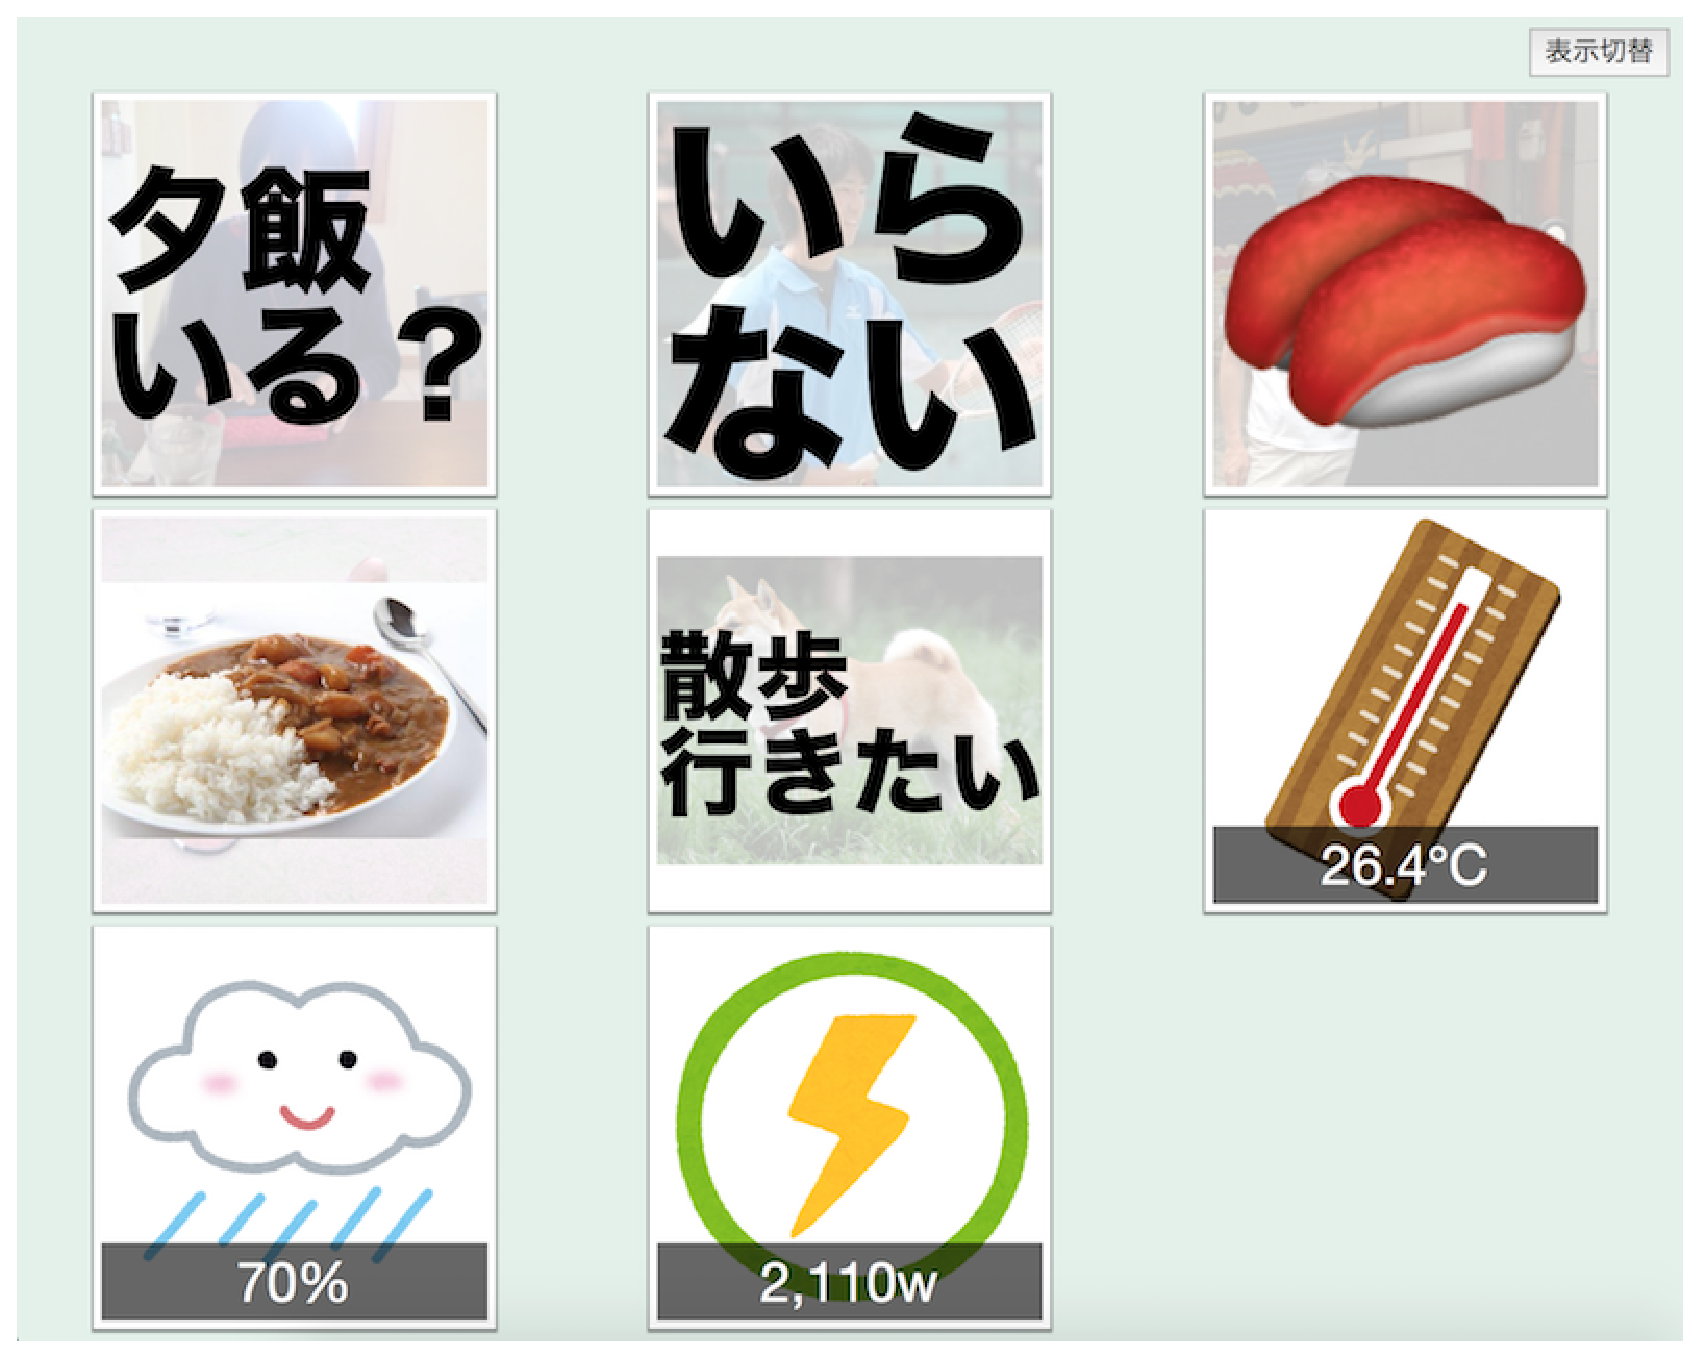
\includegraphics[width=7cm]{images/home.eps}
\caption{家庭での利用}
\label{home}
\end{figure}